\subsection{Problem Overview}

    % \begin{itemize}
    %     \item Why the problem is important.
    %     \item What challenges you need to solve.
    %     \item Which datasets you are planning to use.
    %     \item What metrics you are planning to use to measure your performance.
    % \end{itemize}

Nowadays cameras are available onboard of of almost every new car produced in the last few years. Computer vision provides a very cost effective solution not only to improve safety, but also to one of the holy grails of AI, fully autonomous self-driving cars. 
In this project we are planning to use deep neural networks to solve the object detection and object orientation estimation problems for autonomous driving. 

There are lots of potential challenges that we need to solve for example, 
due to the weather, road conditons and car location, 
images from the car cameras will have a high-variety, which 
requires high robustness for our model. 
And besides the classical object detection task, we 
want to further estimate the 3D orientation from the 2D images.
Last, but not least our 
system need to produce a good result within a limited runtime in order 
to be used in practise.

\subsection{Dataset}
The dataset that we are planning to use is the KITTI Vision Benchmark Suite \cite{Geiger2012CVPR}.  
It's developed for use in mobile robotics and autonomous driving research. So it 
contains several novel challenging benchmarks for the tasks of stereo, optical flow, visual
odometry/SLAM and 3D object detection. 
In our project, we mainly focus on the object detection and orientation estimation task. 
The corresponding benchmark \footnote{\url{http://www.cvlibs.net/datasets/kitti/eval_object.php}} consists of 7481 training images and 7518 test images, comprising a total of 80,256 labeled objects (up to 15 cars and 30 pedestrians are visible per image). All images are color and saved as png.

\JY{Dataset statistics}

\begin{figure}[h!]
\begin{subfigure}{.5\textwidth}
    \centering
    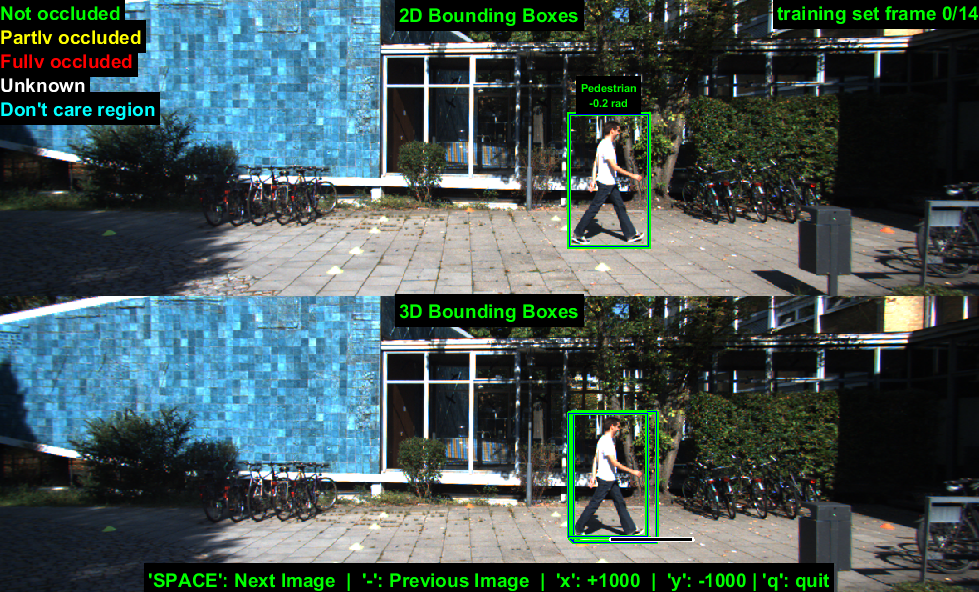
\includegraphics[width=1.0\linewidth]{img/matlab/d1.png}
    % \caption{Seed = 4}
\end{subfigure}%
\begin{subfigure}{.5\textwidth}
    \centering
    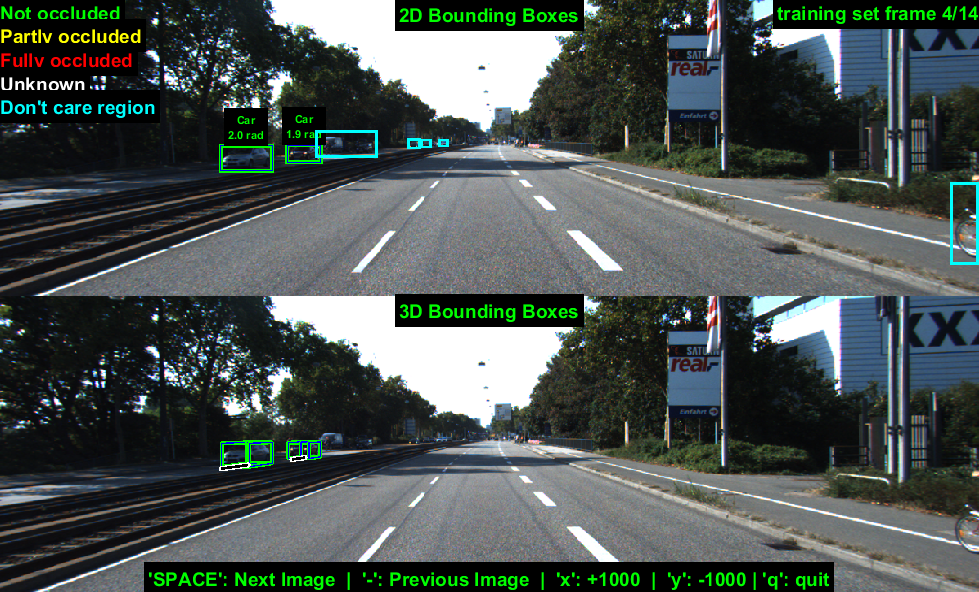
\includegraphics[width=1.0\linewidth]{img/matlab/d5.png}
    % \caption{Seed = 4}
\end{subfigure}
\begin{subfigure}{.5\textwidth}
    \centering
    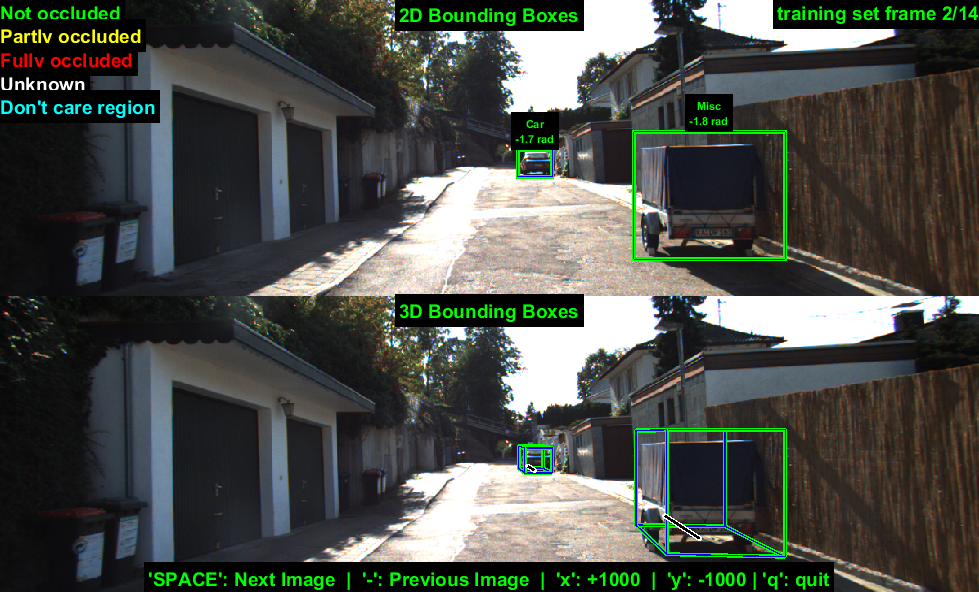
\includegraphics[width=1.0\linewidth]{img/matlab/d3.png}
    % \caption{Seed = 4}
\end{subfigure}%
\begin{subfigure}{.5\textwidth}
    \centering
    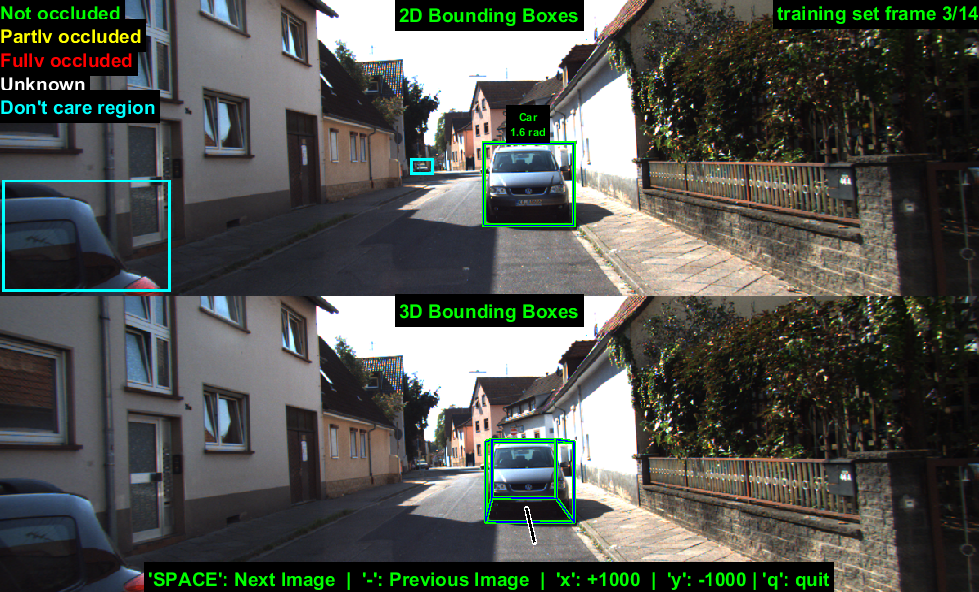
\includegraphics[width=1.0\linewidth]{img/matlab/d4.png}
    % \caption{Seed = 4}
\end{subfigure}
\caption{Some Ground Truth Examples}
\end{figure}

\subsection{Evaluation}

For evaluation, the benchmark is split into three parts: 
First, we need to evaluate the classical
2D object detection by measuring performance using the
well established average precision (AP) metric as described
in \cite{everingham2010pascal}.
Detections are iteratively assigned to ground truth
labels starting with the largest overlap, measured by bounding
box intersection over union. 
True positives are required 
to overlap by more than 50\% and multiple detections
of the same object are counted as false positives. 

Second, we assess the performance
of jointly detecting objects and estimating their 3D
orientation using a novel measure which is called the average
orientation similarity (AOS) \cite{Geiger2012CVPR} and is defined as:
\begin{align}
AOC & = \frac{1}{11} \sum_{r \in \{0,0.1,..,1\}} \max_{\tilde{r}:\tilde{r} \geq r} s(\tilde{r})
\end{align}

Here, $r = \frac{TP}{TP+FN}$ is the PASCAL object detection recall,
where detected 2D bounding boxes are correct if they overlap
by at least 50\% with a ground truth bounding box. The
orientation similarity $s \in [0, 1]$ at recall r is a normalized
($[0..1]$) variant of the cosine similarity defined as
\begin{align}
s(r) & = \frac{1}{|D(r)|} \sum_{i \in D(r)} \frac{1 + cos \Delta_{theta}^{(i)}}{2} \delta_i
\end{align}
where $D(r)$ denotes the set of all object detections at recall
rate 
$r$ and $\Delta_{theta}^{(i)}$
is the difference in angle between estimated
and ground truth orientation of detection $i$. To penalize multiple
detections which explain a single object, we set $\delta_i = 1$
if detection $i$ has been assigned to a ground truth bounding
box (overlaps by at least 50\%) and $\delta_i = 0$ if it has not been
assigned.

Finally, we will also evaluate pure classification (16 bins for
cars) and regression (continuous orientation) performance
on the task of 3D object orientation estimation in terms of
orientation similarity.



